\chapter{Matching Sonar Image Patches}
\label{chapter:matching}

Matching in Computer Vision is the task of deciding whether two images show the same viewpoint of a scene, or contain the same object. The task becomes considerably harder when one has to consider variations in viewpoint, lighting conditions, occlusion, shading, object shape, scale, and background. This problem is similar to Image Registration, where two images are aligned to match their contents. But instead of aligning images, Matching is concerned about a binary decision without resorting to aligning the images. In extreme cases, alignment may not be possible.

Matching is a fundamental problem in Computer Vision \cite{szeliski2010computer}, as it is a vital component of many other tasks, such as stereo vision, structure from motion, and image query/retrieval. Comparison of image patches and prediction of a similarity measure is a common requirement for these

In Robot Perception, Matching is also a fundamental problem with many applications. For example, a Robot might be shown an object and then asked to find it inside a room. This requires the Robot to learn an appropriate representation of the object such as it can be matched to what the Robot is seeing in the scene. Some use cases that requires such functionality are:

\begin{description}
	\item[\textbf{Object Recognition}] \hfill \\
		Given an image, classify its contents into a predefined set of classes. Instead of using a trainable classifier, recognition can be performed by using a database of labeled images and match the input image with one in the labeled database. This approach has the advantage of being dynamic, so new object classes can be easily added to the database, but recognition performance now depends on the quality of the matching functionality.
	\item[\textbf{Object Detection}] \hfill \\
		Similar to Object Recognition, but instead of classifying the complete image, specific objects must be localized in the image. Typically bounding boxes are generated that correspond to the object's localizations in the image.
		Detection can be implemented with Matching by generating candidate locations with a sliding window or a proposal algorithm, and match each of them to a database of labeled images.
	\item[\textbf{Simultaneous Localization and Mapping}] \hfill \\
		SLAM is a fundamental localization problem in Robotics, where a Robot simultaneously builds a map of its environment and localizes itself relative to the map \cite{Cadena16tro-SLAMfuture}. Most SLAM formulations use landmarks in the environment. These landmarks must be tracked and matched to previously seen ones in order for the robot to localize itself, which is a data association problem. This could be done by matching sonar image patches in a underwater SLAM implementation \cite[1em]{hidalgo2015review}.
	\item[\textbf{Tracking}] \hfill \\
		Given a set of images and an object of interest, localize the object in the first image and re-localize the same object in posterior images in the set, even as the object's appearance, background or lighting conditions might change \cite{yilmaz2006object}. Tracking can be implemented by detecting the object of interest in an image, and then detecting candidate objects (through a detection proposal algorithm) and match candidates with the initial tracking target.
\end{description}

While many of the use cases described in this chapter are a field on its own, with mature techniques, using matching to perform such tasks does offer some potential advantages:

\begin{itemize}
	\item Most modern techniques use Machine Learning, and in general, after training an ML model it is difficult to add new data or classes to the model. Normally any model modification requires retraining, which is computationally expensive. Using image matching does not require task-specific training.
	\item Depending on the performance of the matching function, it could better generalize to unseen data, when compared to methods that are trained to specific datasets. One example are keypoint matching methods like SIFT \cite[-3em]{lowe2004distinctive} and SURF \cite[1em]{bay2006surf}, which have been used in many different domains with varying success.
	\item For practical purposes, any useful image matching function can match objects that have never been seen before, which potentially can increase task robustness.
\end{itemize}

For images produced by sonar, matching is currently an open problem. Descriptors and keypoint detectors designed for color images have been previously used for sonar images, but in general they perform poorly. This is expected, as color/optical images are radically different from the acoustic images produced by a sonar.

In this chapter we introduce the use of CNNs to match patches extracted from a sonar image. We formulate the matching problem as binary classification or regression of a similarity score. We show that using CNNs for matching with this setup considerably improves matching performance, moving it from close-to-random-chance to over $90$ \% chance that the correct matching decision will be made. This means that matching as similarity or binary decisions is now usable for real world applications.

\section{Related Work}

Reliably matching sonar images has been an open problem for a long time, but not many publications mention it. It is well known that matching sonar image is considerably more difficult than other kinds of images \cite{negahdaripour2011dynamic}, due to the unique properties of acoustic sensing.

The first approaches to match sonar images use keypoint-based algorithms \cite[1em]{szeliski2010computer}. Many computer vision problems require finding "interesting" or relevant points in an input image, in order to perform tasks such as image alignment and object recognition. The idea of such points is that they are inherent properties of the image, the objects in the image, and/or the environment. These salient features of the image are typically invariant to many transformations, making them very powerful. 

A keypoint is just one of these salient or interesting points in the image, but defining such kind of points in an algorithmic way is not easy. One of the most simple approaches is to detect corners in the image via the Harris corner operator.

Once a keypoint has been detected, in order to be able to find the same keypoint in another image (potentially a different view of the object/scene), a way to match such keypoints must be devised. The most typical approach is to extract a feature vector from the neighbourhood of the keypoint position, and store it in order to perform distance-based matching. Then if many keypoints match across two images, a matching decision can be made by imposing a threshold on this number of matches. This is a very simple but popular approach.

Scale Invariant Feature Transform (SIFT), introduced by David Lowe \cite{lowe2004distinctive}, is one of the first keypoint algorithms that provides reliable matching across different viewpoints of the scene. SIFT uses a scale space ($\sigma$) representation of the image, computed as Difference of Gaussians (DoG), in order to approximate the Laplacian of Gaussians function. The input image $I$ is blurred using a Gaussian filter $G$ at different scales forming a sub-octave. Adjacent sub-octave levels are subtracted to produce the DoG images, and then the input image is down-sampled and the process repeated, producing a Difference of Gaussian Pyramid. Finding keypoints at multiple scales introduces a degree of scale invariance.

\begin{align}
	D(x, y, \sigma) &= L(x, y, \sigma) - L(x, y, \beta \sigma)\\
	L(x, y, \sigma) &= G(x, y, \sigma) * I(x, y)
\end{align}

Then in scale space keypoints are found by comparing the DoG values $D(x, y, \sigma)$, both spatially and in scale (26 neighbours), to the pixel in the centre. If it is an extrema (either a minimum or maximum) then that spatial location is selected as a potential keypoint. Final keypoints are determined by a stability criteria (removing low contrast, noisy and edge keypoints), and interpolated to a more accurate location by using a second-order Taylor expansion.

Then each keypoint is assigned a dominant orientation by estimating the most common gradient orientation around a neighbourhood of the keypoint. This makes sure the descriptor is approximately orientation invariant. Then the image at the detected keypoint scale is rotated around the dominant orientation and a histogram descriptor is computed, producing a 128-element normalized vector.

While SIFT is very popular for color images, its performance on sonar images is quite poor. Some publications \cite[-2em]{vandrish2011side} claim that it works reliably on their data and task, but our own results show that it works quite poorly on our forward-looking sonar data.

SURF \cite[1em]{bay2006surf} is an approximate algorithm based on SIFT, with the aims of a faster implementation. SURF uses averaging filters as an approximation to the Gaussian filters, as it can be implemented with integral images, massively improving performance. The feature vector is computed as the sum of Haar wavelets, which also can be efficiently computed using integral images.

Many publications related to matching sonar images concentrate on slightly different problems, such as mosaicing and image registration. Mosaicing is a popular application of interest point matching, specially in sonar images, that requires registering two or more images accurately in order to blend image pixels, as the image overlap can be used to obtain average pixel values, which decrease sonar image noise and can reveal underlying structure hidden by noise \cite{hurtos2014real}. This operation does require binary matching decisions, but most research work concentrates on the application rather than the technique.

Kim et al. \cite[1em]{kim2005mosaicing} uses the Harris Corner detector to detect feature points on a side-scan sonar image, for the task of matching interest points in two images in order to register them to build a mosaic. After detecting interest points, these are matched between images using a cross-correlation operation (Eq \ref{sic:ccSimilarityEq}) and a minimum feature matching threshold. This approach is generally based on Zhang et al. \cite{zhang1995robust}. The difference between the two techniques is that Kim et al. uses an adaptive threshold based on the $k$-th percentile, while Zhang et al. uses a direct threshold of the correlation score. Both techniques seem to work appropriately to build mosaics, specially as Kim et al. uses RANSAC to estimate a transformation between the images. Note that patch matching for registration in general is not hard, as the transformations between the two images are usually small, as they typically correspond to consecutive image frames in a stream of images produced by the sensor.

Negahdaripour et al. \cite{negahdaripour2011dynamic} also performed matching for image registration with the purpose of mosaicing forward-looking sonar images. Their technique is not fully explained in their paper, and it is described as performing shadow analysis to classify between seafloor and water-column objects, followed by identification of stationary and moving objects. Stationary objects are clustered and their features are used to compute inliers for image registration. Keypoints and used features are based on SIFT. This work good looking mosaics, but as the authors mention, it requires a lot of domain specific knowledge to produce good results, and many parts of the pipeline are hard to train and implement, specially finding moving objects and determining which parts of the image correspond to the seafloor.

Vandrish et al. \cite[-2em]{vandrish2011side} has compared different kinds of registration methods, broadly categorized into global methods, feature-based, and hybrid approaches. Two global methods were evaluated mutual information and phase correlation. The mutual information between two random variables $X$ and $Y$ is:

\begin{align}
	I(X, Y) &= H(X) + H(Y) - H(X, Y)\\		
	H(X) 	&= -\sum_{x \in X} p(x) \log(p(x))\\
	H(X, Y) &= -\sum_{x, y \in X, Y} p(x, y) \log(p(x, y))
\end{align}

Where $H(X)$ is the entropy of $X$ and $H(X, Y)$ is the joint entropy of $X$ and $Y$. This method then tries to find a transformation $T$ that maximizes $I(X, T(Y))$. The authors claim that when the images are maximally aligned, the mutual information is also maximized. The authors mention that this method is very slow, and that it fails if the image pairs do not share enough intensity variation, specially in areas where the background is homogeneous.

Phase Correlation registration works by computing the cross-power spectrum of two images $X$ and $Y$:

\begin{equation}
	e^{j2\pi(\beta u_o + \nu v_0)} = \frac{F_X(\beta, \nu)F^{*}_Y(\beta,\nu)}{||F_X(\beta, \nu)F_Y(\beta,\nu)||}
	\label{mat:cpSpectra}
\end{equation}

Where $F_s$ is the Fourier transform of $s$. This equation comes from the Fourier shift theorem, associating the Fourier transforms of two images that are related by a spatial shift $(u_o, v_o)$ with a constant multiplicative factor. The phase correlation function is computed as the inverse Fourier transform of Eq \ref{mat:cpSpectra}. This function will have a peak at $(u_o, v_o)$, and by finding the maxima it is possible to recover this shift. For the case of a rotation and a translation, the same principle applies, as the spectra is also rotated. To recover the rotation shift, the same method can be applied to the log-polar transformation of the Fourier transform. The authors mention that this method is the most accurate across all evaluated methods. This result is consistent with other publications on the topic \cite{hurtos2014real}.

Only one feature-based registration method was evaluated, corresponding to SIFT. The authors detect SIFT keypoints in both images and try to match their feature descriptors using a nearest neighbour search. The authors experiments show that many false matches are produced in sonar images. RANSAC is applied to discard outliers while fitting a transformation to align both images. The results are good but only when a large number of keypoints are detected. The method fails when keypoints are sparse or when they are mismatched, requiring methods that iteratively refine the learned transformation parameters.

Two hybrid methods were evaluated. The first is a combination of the log-polar transformation:

\begin{align}
	r 		&= \sqrt{(x - x_c)^2 + (y - y_c)^2}\\
	\theta 	&= \tan^{-1}\left ( \frac{y - y_c}{x - x_c} \right )
\end{align}

Where $(x_c, y_c)$ represents the polar center. This transforms the input images in order to provide some kind of normalization, as image rotations are represented as linear shifts in polar coordinates. Then normalized cross-correlation (as presented previously in Eq \ref{sic:ccSimilarityEq}) is applied to obtain the different shifts by using a sliding window and keeping the transformation parameters that maximize the cross-correlation. The second method is Region-of-Interest detection with a custom operator that detects regions of interest through a variance saliency map. Both methods perform poorly, as the correlation between features in multiple observations is quite low, leading to false matches.

Pham and Gueriot \cite{pham2013guided} propose the use of guided block-matching for sonar image registration. The method we propose in this chapter could be considered similar to the block matching step, as this step just needs to make a binary decision whether two pairs of blocks (image patches) match or not. The authors use a pipeline that first extracts dense features from the image, performs unsupervised segmentation of the image through a Self-Organizing map (SOM) applied on the computer features.
The unsupervised segmentation of the image then is used to aid the block matching process, as only blocks that are similar in feature space according to the SOM will be compared, but this process is unsupervised, which implies that different comparison functions will be learned for each image. Then the final step is to estimate a motion vector from the matched blocks, from where a geometrical transformation for registration can be estimated.

The results from this paper show that it performs considerably faster than standard block matching, but only visual results are provided. The displayed mosaics make sense, showing that standard and guided block matching can recover the correct translation vector, but a more through numerical comparison is needed.

Moving into modern methods for matching, Zagoryuko and Komodakis \cite{zagoruyko2015learning} were one of the first to propose the use of CNNs to learn an image matching function, but they instead learn how to compare image patches, corresponding to predicting a similarity score instead of a plain binary classification. We base our own matching networks on this work.

This work defined several CNN models that can be used for patch matching:

\begin{itemize}
	\item \textbf{Siamese Network}: This is a neural network with two branches, where each branch shares weights \cite{bromley1994signature}, as the idea is to compute a relevant feature vector from the image. The computed feature vectors from each branch are then merged and processed into a decision network that outputs the binary matching decision.
	\item \textbf{Pseudo-Siamese Network}: This is a siamese network but in this case each branch does not share weights. This increases the number of learnable parameters, but the authors do not mention any other advantage or intuitive foundation.
	\item \textbf{Two-Channel Network}: This architecture does not have an intrinsic concept of feature vector, as the two input images are combined channel-wise and this two-channel image is input to a single branch CNN that includes a decision network.
	\item \textbf{Central-Surround Two Stream Network}: This architecture is more complex, as it considers two different spatial resolutions from the input image. This is a combination of the two-channel and siamese architectures. The central stream consists of a central crop of each input image, given to one branch, while the surround stream takes two down-sampled (2x) patches as input. The idea of this architecture is to process multiple scale information at the same time.
	\item \textbf{SPP-based}: This network is based on Spatial Pyramid Pooling \cite{he2014spatial}, which is a pooling technique that can make a CNN accept variable-sized inputs. The basic idea of SPP is that instead of performing pooling with fixed-size regions, the regions are variable sized, but the number of output regions is fixed. This produces a fixed-length pooling output, even as the input size is variable. The authors applied SPP to their networks in order to match variable-size patches.
\end{itemize}

These networks are trained on a dataset presented by Brown et al. \cite{brown2011discriminative}. This dataset contains approximate half million $64 \times 64$ labeled image patches, evenly balanced between positives and negatives, that were captured using real 3D correspondences obtained from multi-view stereo depth. The authors evaluate the ROC curves from binary classification, as well as the false positive ratio at $95$ \% true positive rate. The networks are trained with a L2 regularized hinge loss:

\begin{equation}
	L = \frac{\lambda}{2} ||w|| + \sum_i \max(0, 1 - y_i \hat{y}_i)
\end{equation}

Their results show that the best performing network configuration is the two-channel central-surround one, with a considerably margin over all other configurations. The plain two-channel networks perform slightly worse. As two-channel networks are considerably simpler to implement, this is one choice that we made for our own matching networks in this chapter. These results are quite good, but they seem to only be possible due to the large labeled dataset that is available.

The authors also test their matching networks for wide-baseline stereo on a different dataset, showing superior performance when compared with DAISY \cite{tola2008fast}. These results show that using a CNN for matching is quite powerful and can be used for other tasks. Generalization outside of the training set is quite good.

Zbonar and LeCun \cite[1em]{zbontar2016stereo} also propose the use of a CNN to compare image patches. Their method is specifically designed for wide-baseline stereo matching. Given a stereo disparity map, the authors construct a binary classification dataset by extracting one positive and one negative example where true disparity is known a priori.

The authors evaluate two kinds of CNN architectures. The fast architecture is a siamese network with a dot product (cosine) similarity computed between features produced by each branch, while the accurate architecture uses several fully connected layers where the input is a concatenation of the feature vectors produced by each branch. The networks are trained with a hinge loss.

The raw decisions from the CNN models are not good to produce accurate disparity maps, so additional post-processing is used to produce good results. This method was evaluated on the KITTI dataset, and the leaderboard as by October 2015 showed that it was the best performing method, with an error rate of $2.43$ \% with the accurate architecture, and $2.78$ \% with the fast one.

Finally, there is also an application of CNNs to learn keypoint detection, as the Learned Invariant Feature Transform (LIFT) by Yi et al. \cite[-5em]{yi2016lift}. This method train a CNN with four different stages that detect keypoints by producing a dense score map. Keypoints are selected by using a \textit{softargmax} function that finds the maxima of the score map. A spatial transformer network \cite[-3em]{jaderberg2015spatial} is then used to crop a patch from the input image, in the position given by the maxima in the score map.
Then a orientation estimation network estimates the orientation of the image patch, in order to normalize and introduce a degree of orientation invariance. The estimated orientation is then used by a second spatial transformer network to produce a normalized patch that is input to a description network, which outputs a feature vector.

This method mimics the standard SIFT-like feature detection and description pipelines, but the big difference is that all operations are fully differentiable and the whole pipeline can be trained end-to-end. The authors do mention that given the data they had, end-to-end training failed, but training different parts in a hierarchical way. First the descriptor is trained, then the orientation estimator given the descriptor, then the detector given the two previous parts. Different loss functions are used to train the various components in the pipeline.

LIFT was evaluated against classic keypoint detectors, namely SIFT, SURF, ORB, etc. In matching scores, LIFT outperforms all methods by a considerably margin. LIFT obtains matching scores $0.317-0.374$, while SIFT obtains $0.272-0.283$, SURF gets $0.208-0.244$ and ORB performs poorly at $0.127-0.157$. When considering repeatability LIFT obtains $0.446$ while SIFT gets $0.428$. The nearest neighbours area under the Precision-Recall curve is $0.686$ (SIFT obtains $0.517$).

While we do not use LIFT, we believe that it is a major milestone in keypoint detection and feature matching, as this method can learn domain and sensor specific features that could significantly improve the performance of SIFT-like algorithms in sonar images. Training such a method probably requires large quantities of data, and special labels, but it is a clear future direction.

\subsection{Discussion}

While there is a rich literature on mosaicing and registration for sonar images, these approaches typically use simplistic method for image patch matching. The most complex technique that is commonly used is SIFT, which was not designed specifically for sonar images.

Many techniques use extensive domain knowledge in order to obtain good registration performance, but in general evaluation is quite simplistic. Only visual confirmation that the method works in a tiny dataset (less than 10 images) and no further numerical comparison is performed. This is common in the marine robotics community, but that does not mean it is right.

We have not found any technique working on sonar that is similar to the work presented in this chapter. Most research is concentrated around mosaicing and registration, and no other applications that could profit from comparing sonar image patches have been explored. This can easily be explained by the lack of techniques that can reliably match sonar image patches. SIFT and other keypoint matching methods perform poorly according to our own experiments (presented later in Table \ref{mat:matchingResultsTable}). Use of such techniques will produce results that are not publishable.

Our evaluation of CNN-based methods for matching shows that this approach is promising. While it has been applied for tasks that are not common in underwater domains (stereo vision for example), we believe that it can trigger the development of new applications. As we have previously mentioned, object detection and recognition without training sets, SLAM, and Tracking can all benefit from such technique.

\section{Dataset Construction and Preprocessing}

As we do not possess a dataset that is specifically collected and built to train an patch matching algorithm, we decided to build our own from the classification dataset that we possess.

Exploiting the fact that we captured a small set of objects from multiple views, we use this fact to produce synthetic matching pairs where the matching label (positive or negative) can be deduced from the classification class labels. Note that this is not the best way to produce such a dataset. For example, using an additional distance sensor can be used to obtain precise matching labels to produce a much larger dataset. This approach has been used by Aanaes et al. \cite{aanaes2012interesting} to evaluate keypoints detectors, but we have not taken such approach as it is costly and requires a special experimental setup.

We generate three kinds of matching pairs:

\begin{description}
	\item[\textbf{Positive Object-Object}] A positive match pair is constructed from two randomly sampled objects that share a class label. Each object crops can typically correspond to different perspectives of the same object or different insonification levels from the sonar sensor.
	\item[\textbf{Negative Object-Object}] A negative match pair is constructed from two randomly sampled objects that have different class labels.
	\item[\textbf{Negative Object-Background}] A negative match pair is constructed from one randomly sampled object and another randomly sampled background patch with IoU score less than 0.1 with ground truth. We assume that all objects in the dataset are labeled and there is only a small chance that a random background patch might contain an object.
\end{description}

The number of negative match pairs is unbounded, specially for object-background pairs. As a balanced dataset is preferred, we equalize the number of positive and negative matching pairs. To build our dataset, for each labeled object we samples 10 positive object matches, 5 negative object matches, and 5 negative background matches. We use $96 \times 96$ image crops to construct our pairs.

In order to evaluate the generalization ability of our models, we built two datasets, one that shares objects between all splits (train, test and validation), and one that does not share objects. Dataset D (different objects) contains 47280 image pairs, while Dataset S (same objects) contains 54720 image pairs. We split these datasets as $70$ \% training, $15 $ \% validation and $15$ \% testing.

\begin{figure*}
	\centering
	\subfloat[Object-Object Positive Matches]{
		\parbox{0.98\textwidth}{
			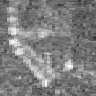
\includegraphics[width=0.11 \textwidth]{chapters/images/matching/match3-A.jpg}
			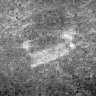
\includegraphics[width=0.11 \textwidth]{chapters/images/matching/match3-B.jpg} \;
			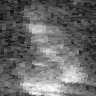
\includegraphics[width=0.11 \textwidth]{chapters/images/matching/match29595-A.jpg}
			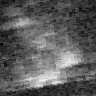
\includegraphics[width=0.11 \textwidth]{chapters/images/matching/match29595-B.jpg} \;
			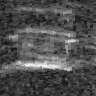
\includegraphics[width=0.11 \textwidth]{chapters/images/matching/match34575-A.jpg}
			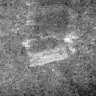
\includegraphics[width=0.11 \textwidth]{chapters/images/matching/match34575-B.jpg}
            
			\vspace*{0.3cm}
            
			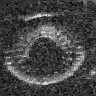
\includegraphics[width=0.11 \textwidth]{chapters/images/matching/match70446-A.jpg}
			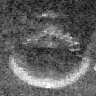
\includegraphics[width=0.11 \textwidth]{chapters/images/matching/match70446-B.jpg} $\;$
			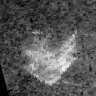
\includegraphics[width=0.11 \textwidth]{chapters/images/matching/match125700-A.jpg}
			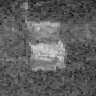
\includegraphics[width=0.11 \textwidth]{chapters/images/matching/match125700-B.jpg} $\;$
			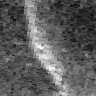
\includegraphics[width=0.11 \textwidth]{chapters/images/matching/match127401-A.jpg}
			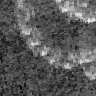
\includegraphics[width=0.11 \textwidth]{chapters/images/matching/match127401-B.jpg}
		}	
	}

	\subfloat[Object-Object Negative Matches]{
		\parbox{0.98\textwidth}{
			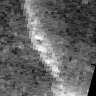
\includegraphics[width=0.11 \textwidth]{chapters/images/matching/non-match126939-A.jpg}
			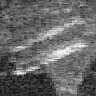
\includegraphics[width=0.11 \textwidth]{chapters/images/matching/non-match126939-B.jpg} \;
			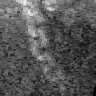
\includegraphics[width=0.11 \textwidth]{chapters/images/matching/non-match129879-A.jpg}
			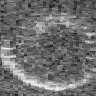
\includegraphics[width=0.11 \textwidth]{chapters/images/matching/non-match129879-B.jpg} \;
			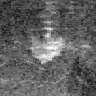
\includegraphics[width=0.11 \textwidth]{chapters/images/matching/non-match137556-A.jpg}
			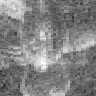
\includegraphics[width=0.11 \textwidth]{chapters/images/matching/non-match137556-B.jpg}
            
			\vspace*{0.3cm}
            
			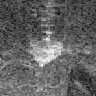
\includegraphics[width=0.11 \textwidth]{chapters/images/matching/non-match139410-A.jpg}
			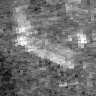
\includegraphics[width=0.11 \textwidth]{chapters/images/matching/non-match139410-B.jpg} \;
			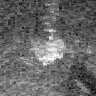
\includegraphics[width=0.11 \textwidth]{chapters/images/matching/non-match141822-A.jpg}
			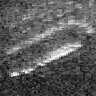
\includegraphics[width=0.11 \textwidth]{chapters/images/matching/non-match141822-B.jpg} \;
			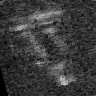
\includegraphics[width=0.11 \textwidth]{chapters/images/matching/non-match44796-A.jpg}
			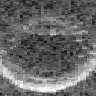
\includegraphics[width=0.11 \textwidth]{chapters/images/matching/non-match44796-B.jpg}
		}
	}

	\subfloat[Object-Background Negative Matches]{
		\parbox{0.98\textwidth}{
			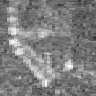
\includegraphics[width=0.11 \textwidth]{chapters/images/matching/non-match-bg45-A.jpg}
			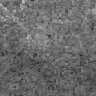
\includegraphics[width=0.11 \textwidth]{chapters/images/matching/non-match-bg45-B.jpg} \;
			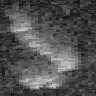
\includegraphics[width=0.11 \textwidth]{chapters/images/matching/non-match-bg17508-A.jpg}
			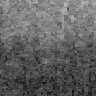
\includegraphics[width=0.11 \textwidth]{chapters/images/matching/non-match-bg17508-B.jpg} \;
			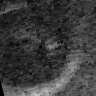
\includegraphics[width=0.11 \textwidth]{chapters/images/matching/non-match-bg17571-A.jpg}
			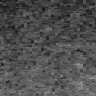
\includegraphics[width=0.11 \textwidth]{chapters/images/matching/non-match-bg17571-B.jpg}
            
			\vspace*{0.3cm}
            
			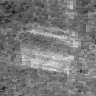
\includegraphics[width=0.11 \textwidth]{chapters/images/matching/non-match-bg32877-A.jpg}
			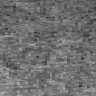
\includegraphics[width=0.11 \textwidth]{chapters/images/matching/non-match-bg32877-B.jpg} \;
			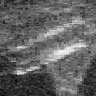
\includegraphics[width=0.11 \textwidth]{chapters/images/matching/non-match-bg75168-A.jpg}
			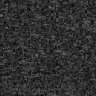
\includegraphics[width=0.11 \textwidth]{chapters/images/matching/non-match-bg75168-B.jpg} \;
			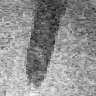
\includegraphics[width=0.11 \textwidth]{chapters/images/matching/non-match-bg90705-A.jpg}
			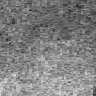
\includegraphics[width=0.11 \textwidth]{chapters/images/matching/non-match-bg90705-B.jpg}
		}
	}
	\vspace*{0.5cm}
	\caption[Small sample of sonar image patch pairs generated by our methodology]{Small sample of sonar image patch pairs generated by our methodology. One positive match class and two negative match classes are displayed.}
	\label{mat:datasetPatchSamples}
\end{figure*}

\FloatBarrier
\section{Matching with CNNs}

In this chapter we propose the use of Convolutional Neural Networks to match two image patches of the same size. Most of our work is inspired by the work of Zagoryuko and Komodakis \cite{zagoruyko2015learning}, as they introduced the use of CNNs for patch comparison. 

We framed the matching problem as both a classification and a regression problem. The idea is that a classification problem will fit a model to the true class labels, but additionally this model could produce probability scores (through a softmax activation function) that could aid in the matching decision process. A natural extension would be to regress these scores directly from the class labels. These scores then could be thresholded to produce binary matching decisions.

We evaluated two different CNN architectures. One is a siamese CNN with two branches, and the other is a simple feed-forward CNN that receives a two-channel input image.

The two-channel CNN was originally introduced by Zagoryuko and Komodakis. Our incarnation of that model is shown in Figure \ref{mat:twoChanCNN}. As matching uses two images as inputs, this network takes a two-channel input image. This is constructed by just concatenating the two $96 \times 96$ sonar image patches along the channels dimension into $2 \times 96 \times 96$ tensor.

All layers use the ReLU activation, except for the output layer. Dropout \cite{srivastava2014dropout} with $p = 0.5$ is used in the two first fully connected layers in order to reduce overfitting and improve generalization performance.

For matching as classification, we use $c = 2$ as it corresponds to a binary classification problem. A softmax activation function is used at the output fully connected layer. In this configuration the network has 126513 parameters (with a parameter to data points ratio of $\frac{126513}{33096} \sim 3.8$, reduced to $1.9$ with Dropout at training time). This model is trained with a categorical cross-entropy loss function.
For matching as regression, we use $c = 1$ and a sigmoid activation at the output fully connected layer. This network configuration has 125K parameters (with a parameter to data points ratio of $\frac{125000}{33096} \sim 3.7$, reduced to $1.8$ with Dropout at training time). This model is trained with a binary cross-entropy layer (Equation \ref{mat:binaryCELoss}) which is just the scalar output version of the categorical cross-entropy. We also tried other losses such as mean average error (L1 loss), mean squared error (L2 loss) and smooth L1 loss, but they were not any enhancement over the binary cross-entropy.

\begin{equation}
	L(y, \hat{y}) = - \sum_i y_i \log(\hat{y}_i) = -y_0 \log(\hat{y}_0) - (1 - y_0) \log(1 - \hat{y}_0)
	\label{mat:binaryCELoss}
\end{equation}

The Siamese CNN architecture is shown in Figure \ref{mat:siameseCNN}. Unlike the previous network, this model takes two $96 \times 96$ input images separately. Each branch of the siamese network shares weights. The basic idea of this model is that each branch extracts relevant features from each image, and weight sharing allows for a reduction in the number of parameters, as well as making sure that invariant and equivalent features are extracted from each image.

Both networks are trained in the same way, using ADAM as optimizer with initial learning rate $\alpha = 0.01$ and batch size $B = 128$ elements. The two-channel CNN model is trained for $M = 5$ epochs, while the Siamese CNN model is trained for $M = 15$ epochs.

\begin{marginfigure}
    \centering
    \begin{tikzpicture}[style={align=center, minimum height=0.5cm, minimum width=2.5cm}]		
    \node[draw] (A) {FC(c)};	
    
    \node[above=1em of A] (output) {Match\\Decision};
    
    \node[above=1 em of output] (dummy) {};
    \node[draw, below=1em of A] (B) {FC(32)};
    \node[draw, below=1em of B] (C) {FC(64)};
    
    \node[draw, below=1em of C] (D) {MaxPool(2, 2)};f
    \node[draw, below=1em of D] (E) {Conv($16$, $5 \times 5$)};
    
    \node[draw, below=1em of E] (F) {MaxPool(2, 2)};
    \node[draw, below=1em of F] (G) {Conv($32$, $5 \times 5$)};
    
    \node[draw, below=1em of G] (H) {MaxPool(2, 2)};
    \node[draw, below=1em of H] (I) {Conv($32$, $5 \times 5$)};
    
    \node[draw, below=1em of I] (J) {MaxPool(2, 2)};
    \node[draw, below=1em of J] (K) {Conv($16$, $5 \times 5$)};	
    
    \node[below=1em of K] (Input) {Two-Channel\\Input Image};	
    
    \draw[-latex] (B) -- (A);
    \draw[-latex] (C) -- (B);
    \draw[-latex] (D) -- (C);
    \draw[-latex] (E) -- (D);
    \draw[-latex] (F) -- (E);
    \draw[-latex] (G) -- (F);
    \draw[-latex] (H) -- (G);
    \draw[-latex] (I) -- (H);
    \draw[-latex] (J) -- (I);
    \draw[-latex] (K) -- (J);
    \draw[-latex] (Input) -- (K);
    \draw[-latex] (A) -- (output);
    \end{tikzpicture}
    \caption{CNN architecture for matching using a two-channel input image}
    \label{mat:twoChanCNN}
\end{marginfigure}

\begin{figure}[p]
	\vspace*{1.0cm}
	\centering
	\begin{tikzpicture}[style={align=center, minimum height=0.7cm, minimum width=2.7cm}]
	
	\node[] (dummy) {};
	
	\node[draw, above=2em of dummy] (merge) {Merge};
	\node[draw, above=1em of merge] (fc1) {FC(64)};
	\node[draw, above=1em of fc1] 	(fc2) {FC(c)};
	
	\node[above=1em of fc2] 	(output) {Match\\Decision};
	
	\node[draw, left=0.5em of dummy] (upB) {FC(96)};
	\node[draw, below=1em of upB] (upC) {FC(96)};
	
	\node[draw, below=1em of upC] (upD) {MaxPool(2, 2)};
	\node[draw, below=1em of upD] (upE) {Conv($16$, $5 \times 5$)};
	
	\node[draw, below=1em of upE] (upF) {MaxPool(2, 2)};
	\node[draw, below=1em of upF] (upG) {Conv($32$, $5 \times 5$)};
	
	\node[draw, below=1em of upG] (upH) {MaxPool(2, 2)};
	\node[draw, below=1em of upH] (upI) {Conv($32$, $5 \times 5$)};
	
	\node[draw, below=1em of upI] (upJ) {MaxPool(2, 2)};
	\node[draw, below=1em of upJ] (upK) {Conv($16$, $5 \times 5$)};	
	
	\node[draw, right=0.5em of dummy] (downB) {FC(96)};
	\node[draw, below=1em of downB] (downC) {FC(96)};
	
	\node[draw, below=1em of downC] (downD) {MaxPool(2, 2)};
	\node[draw, below=1em of downD] (downE) {Conv($16$, $5 \times 5$)};
	
	\node[draw, below=1em of downE] (downF) {MaxPool(2, 2)};
	\node[draw, below=1em of downF] (downG) {Conv($32$, $5 \times 5$)};
	
	\node[draw, below=1em of downG] (downH) {MaxPool(2, 2)};
	\node[draw, below=1em of downH] (downI) {Conv($32$, $5 \times 5$)};
	
	\node[draw, below=1em of downI] (downJ) {MaxPool(2, 2)};
	\node[draw, below=1em of downJ] (downK) {Conv($16$, $5 \times 5$)};	
	
	\node[below=1em of upK] (inputA) {Input\\Image A};
	\node[below=1em of downK] (inputB) {Input\\Image B};
	
	\draw[-latex] (upC) -- (upB);
	\draw[-latex] (upD) -- (upC);
	\draw[-latex] (upE) -- (upD);
	\draw[-latex] (upF) -- (upE);
	\draw[-latex] (upG) -- (upF);
	\draw[-latex] (upH) -- (upG);
	\draw[-latex] (upI) -- (upH);
	\draw[-latex] (upJ) -- (upI);
	\draw[-latex] (upK) -- (upJ);
	
	\draw[-latex] (downC) -- (downB);
	\draw[-latex] (downD) -- (downC);
	\draw[-latex] (downE) -- (downD);
	\draw[-latex] (downF) -- (downE);
	\draw[-latex] (downG) -- (downF);
	\draw[-latex] (downH) -- (downG);
	\draw[-latex] (downI) -- (downH);
	\draw[-latex] (downJ) -- (downI);
	\draw[-latex] (downK) -- (downJ);
	
	\draw[-latex] (inputA) -- (upK);
	\draw[-latex] (inputB) -- (downK);
	
	\draw[-latex] (upB) -- (merge);
	\draw[-latex] (downB) -- (merge);
	\draw[-latex] (merge) -- (fc1);
	\draw[-latex] (fc1) -- (fc2);
	
	\draw[-latex] (fc2) -- (output);
	\end{tikzpicture}
	\vspace*{0.5cm}
	\caption{Siamese CNN architecture for matching using a two one-channel input images}
	\label{mat:siameseCNN}
\end{figure}

\section{Experimental Evaluation}

\subsection{Evaluation Metrics}

Matching is a fundamentally different problem from multi-class image classification, as we have modeled matching as a binary classification problem. This defines a different set of candidate metrics: false and true positive rates, precision and recall, ROC curves, and accuracy \cite{bishop2006pattern}.

From the Marine Debris task point of view, it is desirable that the matching algorithm produces a quantifiable measure of similarity or confidence, so it can be interpreted by a human. Metrics that prefer binary results like \textit{match} or \textit{no match} without an explanation by similarity or confidence score are not as useful as ones that evaluate confidence in the decision that was made.

For this reason we chose the area under the ROC curve (AUC) as primary evaluation metric. This measures the confidence score quality produced by the classifier \cite{murphy2012machine}. Classifiers that receive higher AUC values produce confidence scores that are better separate classes, so a simple threshold on the score can be used to make class decisions. The ROC curve, and consequently the AUC, incorporate the precision and recall metrics in its calculation.

\subsection{Model Comparison}

In this section we evaluate our CNNs for matching with state of the art keypoint matching algorithms, and we also evaluate some baselines based on classic machine learning algorithms trained on our datasets. For keypoint matching we evaluate SIFT, SURF, ORB and AKAZE.

These keypoint detectors are evaluated through a common protocol. Keypoints are detected in each input image and matched using a k-nearest neighbour search with $k = 2$ over the computed descriptors in each keypoint. For continuous features (AKAZE, SIFT, and SURF) we compute the number of "good" matches using the ratio test \cite{lowe2004distinctive}. This test requires at least three matches, and it filters descriptor matches according to the distance ratio between one match and the second-best match. If this ratio is too large, the match is discarded. Then we use the number of "good" matches produced with a ratio threshold of $0.75$ and set a minimum threshold to declare a match between two images.

For binary features (ORB) we only use the number of matches and put a minimum threshold to declare a match between two images. This threshold is used to construct the ROC curve later on.

As machine learning baselines we evaluate:

\begin{description}
	\item[\textbf{Random Forest}] A random forest \cite{murphy2012machine} seems to be a good choice as it is both resistant to overfitting due to the use of an ensemble of decision trees, and it is a learning algorithm with a non-linear decision boundary. We trained a random forest classifier and a random forest regressor. Both share the same hyper-parameters. We used a forest with 30 trees and a maximum depth of 40 levels. Each classification decision tree is trained by minimizing the gini impurity. For regression decision trees, we used the mean squared error. The random forest classifier can provide class probabilities for positive and negative matches as the voting ratio of each leaf.
	
	\item[\textbf{Support Vector Machine}] A support vector machine represents a lower bound on performance, as this learning algorithm is reproducible due to the use of an optimal separating hyperplane. We tried both a support vector machine for classification, and a support vector regressor for regression of the target scores. The SVM is trained with regularization coefficient $C = 1$, while the SVR regressor is trained with $C = 10$ and $\epsilon = 0.05$. The trained SVM includes probability information through the use of internal cross-validation.
\end{description}

Both kinds of ML classifiers were tuned using grid search over a predefined grid of parameters. Keypoint method have no hyper-parameters to be tuned. We now describe our evaluation metrics.

As we model matching as a binary classification problem, we use the Area under the ROC Curve (AUC) as our primary metric. The ROC curve is obtained by computing the true positive (TPR) and false positive rates (FPR):

\begin{equation}
	\text{TPR} = \frac{TP}{P} \qquad \text{FPR} = \frac{FP}{N}
\end{equation}

Assuming a classifier that provides a score for each class, then the TPR and FPR rates vary as a threshold is set on the output classification score. Then the ROC curve is built as points in the $(\text{FPR}, \text{TPR})$ space as the threshold is varied. This curve indicates the different operating points that a given classifier outputs can produce, and it is useful in order to tune a specific threshold while using the classifier in production.

The AUC is the just the area under the ROC curve, which is a number in the $[0, 1]$ range. The AUC is a metric that is not simple to interpret \cite{sammut2011encyclopedia}. One interpretation is that the AUC is the probability that the classifier will produce a higher score for a randomly chosen positive example than a randomly chosen negative example. A classifier with a higher AUC is then preferable.

We also evaluated accuracy, but as we have labels for the three components that were used to generate each dataset, we also evaluated accuracy on each component. This includes examples that represent a object-object positive match, a object-object negative match, and a object-background negative match. We also compute and present mean accuracy. As we are also evaluating regressors to predict a score, we compute accuracy from class predictions:

\begin{equation}
	c = \argmax\{1 - p, p\}
\end{equation}

Where $p$ is the output prediction from the regressor or probability from a classifier. For keypoint detectors we compute accuracies using a threshold equal to zero for the minimum number of matches. This value produces the maximum possible accuracy for these methods.

Numerical results are presented in Table \ref{mat:matchingResultsTable}, while ROC curve plots are shown in Figures \ref{mat:rocSamePlot} and \ref{mat:rocDiffPlot}.

We only evaluated keypoint detection methods on one of the datasets. Their performance is virtually the same and it is not affected by objects in the training set, as these methods do not use learning. Keypoint matching algorithms perform quite poorly, with AUC that is slightly larger than random chance ($0.5$). Their mean accuracy is also quite close to random chance, which is product of very low accuracies in the object-object negative match case. These results show that keypoint methods work at an acceptable performance when matching the same object under a different view (a positive match) but fail to declare a mismatch for different objects (negative matches). Seems that keypoint detection is overconfident and produces too many positive matches, which translates to lower accuracies in the two negative cases.

\begin{table*}[t]
	\forcerectofloat
	\centering
	
	\begin{tabular}{lllllll}
		\hline 
		& Method 	& AUC	 	& Mean Acc & Obj-Obj $+$ Acc 	& Obj-Obj $-$ Acc 	& Obj-Bg $-$ Acc\\ 
		\hline 
		& SIFT	& $0.610$ 	& $54.0 $ \% & $74.5 $ \% 		&  $43.6 $ \%			&  $44.0 $ \% \\
		& SURF	& $0.679$	& $48.1 $ \% & $89.9 $ \% 		&  $18.6 $ \%			&  $35.9 $ \% \\
		& ORB	& $0.682$	& $54.9 $ \% & $72.3 $ \% 		&  $41.9 $ \%			&  $60.5 $ \% \\
		& AKAZE	& $0.634$	& $52.2 $ \% & $95.1 $ \% 		&  $4.8 $ \%				&  $56.8 $ \% \\
		\hline
		
		\multirow{6}{*}{\rotatebox{90}{Different}}& RF-Score	& $0.741$	& $57.6 $ \% & $22.5 $ \% 		&  $88.2 $ \%				&  $97.2 $ \% \\
		& RF-Class	& $0.795$	& $69.9 $ \% & $12.5 $ \% 		&  $\textbf{97.7} $ \%				&  $\textbf{99.7} $ \% \\
		\cline{2-7}
		& SVR-Score	& $0.663$	& $70.5 $ \% & $57.2 $ \% 		&  $66.6 $ \%				&  $87.5 $ \% \\
		& SVM-Class	& $0.652$	& $67.1 $ \% & $54.4 $ \% 		&  $69.1 $ \%				&  $90.5 $ \% \\
		\cline{2-7}		
		& 2-Chan CNN Scr & $0.894$	& $82.9 $ \% & $\textbf{68.0} $ \% &  $96.1 $ \%				&  $84.5 $ \% \\
		& 2-Chan CNN Cls & $\textbf{0.910}$	& $86.2 $ \% & $67.3 $ \% &  $95.2 $ \%				&  $96.1 $ \% \\
		\cline{2-7}
		& Siam CNN Scr & $0.826$	& $77.0 $ \% & $49.2 $ \% &  $84.7 $ \%				&  $97.0 $ \% \\
		& Siam CNN Cls & $0.855$	& $82.9 $ \% & $62.9 $ \% &  $89.9 $ \%				&  $96.0 $ \% \\
		\hline
		
		\multirow{6}{*}{\rotatebox{90}{Same}}& RF-Score	& $0.972$	& $85.2 $ \% & $\textbf{98.7} $ \% 		&  $58.8 $ \%				&  $98.1 $ \% \\
		& RF-Class	& $\textbf{0.982}$	& $90.9 $ \% & $97.3 $ \% 		&  $75.8 $ \%				&  $\textbf{99.6} $ \% \\
		\cline{2-7}
		& SVR-Score	& $0.767$	& $66.2 $ \% & $86.3 $ \% 		&  $17.6 $ \%				&  $94.7 $ \% \\
		& SVM-Class	& $0.742$	& $64.8 $ \% & $83.7 $ \% 		&  $18.3 $ \%				&  $92.4 $ \% \\
		\cline{2-7}		
		& 2-Chan CNN Scr & $0.934$	& $85.4 $ \% & $85.0 $ \% &  $\textbf{77.5} $ \%				&  $93.7 $ \% \\
		& 2-Chan CNN Cls & $0.944$	& $86.7 $ \% & $86.6 $ \% &  $75.7 $ \%				&  $97.8 $ \% \\
		\cline{2-7}		
		& Siam CNN Scr & $0.895$	& $80.6 $ \% & $89.1 $ \% &  $55.3 $ \%				&  $97.3 $ \% \\
		& Siam CNN Cls & $0.864$	& $75.8 $ \% & $92.2 $ \% &  $39.4 $ \%				&  $95.8 $ \% \\
		\hline
	\end{tabular}
	\vspace*{0.5cm}
	\caption[Comparison of different models for matching]{Comparison of different models for matching. Area Under the ROC Curve (AUC), Accuracy at match threshold zero, and Accuracy for each match type is reported for both datasets (Same and Different).}
	\label{mat:matchingResultsTable}
\end{table*}

Machine learning methods perform considerably better. Considering different objects (Dataset D), a Random Forest performs adequately, obtaining AUC in the range $[0.74, 0.79]$, and this method produces very good accuracy for the negative cases, but poor accuracy for the positive match case. Seems a random forest has the opposite behaviour than the keypoint matching algorithms, as it is overconfident on negative matches but performs poorly for the positive ones.

An SVM and SVR both perform quite poorly, with similar AUC close to $0.65$, but a more balanced performance across match cases, but still biased performance towards object-background negative cases.

Our proposed method using a CNN outperforms all other methods in the different objects case. This means that a CNN can learn appropriate features that generalize well outside of the training set, even generalizing to different objects. The best performing network is a two-channel one producing class probabilities, closely followed by also a two-channel network that produces a single regression score that is used for matching. There is a $2$ \% difference in the AUC of these networks.

Siamese networks also perform quite well but below the performance of the two-channel networks. All CNN methods have a common performance pitfall, as negative cases have very good accuracy, but the positive case has lower accuracy, which is approximately $20$ \% over the random chance minimum.

Considering the same objects in the training and testing sets (Dataset S), results change radically. All method perform better than in Dataset D. For this case, the best performing method is a random forest classifier, with $0.982$ AUC. A regression random forest obtains $1$ \% less AUC. Comparing RF performance with that of Dataset D shows that the RF classifier suffers from mild overfitting. It is not memorizing the training set but the learned classifier favours objects in the training set, performing very well on them, but decreasing performance considerably with unseen objects.

Other methods also perform considerably better. An SVM/SVR increases AUC by approximately $10$ \%, but a two-channel CNN only improves AUC by $3$ \%. This suggests that CNN methods are not overfitting and the loss in performance is acceptable for unseen objects.

It seems that as a general pattern, matching as a classification problem produces better results than using a regression problem. Only some exceptions to this pattern occur, such as a Siamese network in Dataset S, and SVR on both datasets.

Our results show that using a CNN is a very good option for the problem of matching pairs of sonar image patches.

\pgfplotsset{cycle list/Set1-6}

\pgfplotscreateplotcyclelist{matiasList}{%
	{color=red,solid},
	{color=blue,solid},
	{color=green,solid},
	{color=black,solid},
	{color=red,densely dashed},
	{color=blue,densely dashed},
	{color=green,densely dashed},
	{color=black,densely dashed},
	{color=red,densely dotted},
	{color=blue,densely dotted},
	{color=green,densely dotted},
	{color=black,densely dotted}}

\begin{figure}[h]
	\begin{tikzpicture}
	\begin{axis}[height = 0.35\textheight, width = 0.7\textwidth, xlabel={False Positive Rate}, ylabel={True Positive Rate}, xmin=0, xmax=1.0, ymin=0, ymax=1.0, ymajorgrids=true, xmajorgrids=true, grid style=dashed, legend pos = outer north east, legend style={font=\scriptsize, at = {(1.1, 1.0)}}, cycle multiindex* list={matiasList}, legend columns = 1]
	\addplot +[no markers, raw gnuplot] gnuplot {
		plot 'chapters/data/matching/different/MatchingCNNDropoutClassNoAugment-DiffObjects-ROCCurve.csv' using 2:3 smooth sbezier;
	};
	\addlegendentry{CNN 2-Chan Class}
	
	\addplot +[no markers, raw gnuplot] gnuplot {
		plot 'chapters/data/matching/different/MatchingCNNDropoutScoreBCENoAugment-DiffObjects-ROCCurve.csv' using 2:3 smooth sbezier;
	};
	\addlegendentry{CNN 2-Chan Score}
	
	\addplot +[no markers, raw gnuplot] gnuplot {
		plot 'chapters/data/matching/different/svmProbsROCCurve.csv' using 2:3 smooth sbezier;
	};
	\addlegendentry{SVM-Class}
	
	\addplot +[no markers, raw gnuplot] gnuplot {
		plot 'chapters/data/matching/different/svrROCCurve.csv' using 2:3 smooth sbezier;
	};
	\addlegendentry{SVR-Score}
	
	\addplot +[no markers, raw gnuplot] gnuplot {
		plot 'chapters/data/matching/different/randomForestClassifierROCCurve.csv' using 2:3 smooth sbezier;
	};
	\addlegendentry{RF-Class}
	
	\addplot +[no markers, raw gnuplot] gnuplot {
		plot 'chapters/data/matching/different/randomForestROCCurve.csv' using 2:3 smooth sbezier;
	};
	\addlegendentry{RF-Score}
	
	\addplot+[mark = none] table[x  = fpr, y  = tpr, col sep = space] {chapters/data/matching/siftMatcherPRCurve.csv};
	\addlegendentry{SIFT}
	\addplot+[mark = none] table[x  = fpr, y  = tpr, col sep = space] {chapters/data/matching/surfMatcherPRCurve.csv};
	\addlegendentry{SURF}
	\addplot+[mark = none] table[x  = fpr, y  = tpr, col sep = space] {chapters/data/matching/orbMatcherPRCurve.csv};
	\addlegendentry{ORB}	
	\addplot+[mark = none] table[x  = fpr, y  = tpr, col sep = space] {chapters/data/matching/akazeMatcherPRCurve.csv};
	\addlegendentry{AKAZE}
	\draw[gray] (axis cs:0,0) -- (axis cs:1,1);
	\end{axis}        
	\end{tikzpicture}
	\caption[ROC curve comparing different methods for sonar image patch matching on Dataset D]{ROC curve comparing different methods for sonar image patch matching on Dataset D, meaning different objects were used to produce the training and testing sets. The grey line represents random chance limit.}
	\label{mat:rocDiffPlot}
\end{figure}

\begin{figure}[h]
	\begin{tikzpicture}
	\begin{axis}[height = 0.35\textheight, width = 0.7\textwidth, xlabel={False Positive Rate}, ylabel={True Positive Rate}, xmin=0, xmax=1.0, ymin=0, ymax=1.0, ymajorgrids=true, xmajorgrids=true, grid style=dashed, legend pos = outer north east, legend style={font=\scriptsize, at = {(1.1, 1.0)}}, cycle multiindex* list={matiasList}, legend columns = 1]
	\addplot +[no markers, raw gnuplot] gnuplot {
		plot 'chapters/data/matching/same/MatchingCNNDropoutClassNoAugment-SameObjects-ROCCurve.csv' using 2:3 smooth sbezier;
	};
	\addlegendentry{CNN 2-Chan Class}
	
	\addplot +[no markers, raw gnuplot] gnuplot {
		plot 'chapters/data/matching/same/MatchingCNNDropoutScoreBCENoAugment-SameObjects-ROCCurve.csv' using 2:3 smooth sbezier;
	};
	\addlegendentry{CNN 2-Chan Score}
	
	\addplot +[no markers, raw gnuplot] gnuplot {
		plot 'chapters/data/matching/same/svmProbsROCCurve.csv' using 2:3 smooth sbezier;
	};
	\addlegendentry{SVM-Class}
	
	\addplot +[no markers, raw gnuplot] gnuplot {
		plot 'chapters/data/matching/same/svrROCCurve.csv' using 2:3 smooth sbezier;
	};
	\addlegendentry{SVR-Score}
	
	\addplot +[no markers, raw gnuplot] gnuplot {
		plot 'chapters/data/matching/same/randomForestClassifierROCCurve.csv' using 2:3 smooth sbezier;
	};
	\addlegendentry{RF-Class}
	
	\addplot +[no markers, raw gnuplot] gnuplot {
		plot 'chapters/data/matching/same/randomForestROCCurve.csv' using 2:3 smooth sbezier;
	};
	\addlegendentry{RF-Score}
	
	\addplot+[mark = none] table[x  = fpr, y  = tpr, col sep = space] {chapters/data/matching/siftMatcherPRCurve.csv};
	\addlegendentry{SIFT}
	\addplot+[mark = none] table[x  = fpr, y  = tpr, col sep = space] {chapters/data/matching/surfMatcherPRCurve.csv};
	\addlegendentry{SURF}
	\addplot+[mark = none] table[x  = fpr, y  = tpr, col sep = space] {chapters/data/matching/orbMatcherPRCurve.csv};
	\addlegendentry{ORB}	
	\addplot+[mark = none] table[x  = fpr, y  = tpr, col sep = space] {chapters/data/matching/akazeMatcherPRCurve.csv};
	\addlegendentry{AKAZE}
	\draw[gray] (axis cs:0,0) -- (axis cs:1,1);
	\end{axis}        
	\end{tikzpicture}
	\caption[ROC curve comparing different methods for sonar image patch matching on Dataset S]{ROC curve comparing different methods for sonar image patch matching on Dataset S, meaning the same objects were used to produce the training and testing sets. The grey line represents random chance limit.}
	\label{mat:rocSamePlot}
\end{figure}

\FloatBarrier
\subsection{How Much Data is Needed?}

In this section we explore the question of how generalization varies with training set size. We use the same basic methodology as previously mentioned in Section \ref{lim:secNumTrainingSamples}. We only evaluated the two-channel networks, as they performed the best.

We vary the number of samples per class (SPC) from 1 to 5000. The original training set contains approximately 40000 samples which corresponds to a SPC of 20000. Due to computational constraints we only evaluate up to SPC 5000. As like our previous evaluations of matching algorithms, we evaluate the area under the curve (AUC) for each data point.

Results are presented in Figure \ref{mat:spcVsAUC}. Both scoring and classification networks perform quite similarly as the training set size is varied. But the classification network gets slightly better AUC performance with low sample quantity. This can be seen as the classifier obtaining performance that is slightly better than random chance ($50$ \%) at one sample per class, while the scorer obtains worse than random chance performance at the same SPC value.

As SPC increases, performance increases rapidly for SPC less than 750, and after that the increases are smaller (diminishing returns). Both models converge after SPC 5000 close to $90$ \% AUC. This shows that the full dataset is required to produce good generalization performance, and these networks do not perform well if only a smaller dataset is available.

These results are consistent with the difficulty of matching sonar image patches. It seems the only way to improve these models is to increase the size of the training set, as with many other ML algorithms. But we also believe that other approaches could work better, specially the ones from fields like one-shot learning. One natural choice would be a network with a contrastive or triplet loss \cite{Schroff_2015_CVPR}. This kind of networks is trained in a different way, where an embedding is learned in such a way to maximize embedded distances between negative samples, and minimize the distances between positive examples. This makes a much more discriminative model.

\begin{figure*}[!ht]
	\forcerectofloat
	\centering
	\begin{tikzpicture}
	\begin{customlegend}[legend columns = 4,legend style = {column sep=1ex}, legend cell align = left,
	legend entries={CNN 2-Chan Class, CNN 2-Chan Score}]
	\addlegendimage{mark=none,blue}
	\addlegendimage{mark=none,red}
	\end{customlegend}
	\end{tikzpicture}
	
	\subfloat[Sub-Region $1-500$]{
		\begin{tikzpicture}
		\begin{axis}[
		xlabel={Samples per Class},
		ylabel={Test AUC (\%)},        
		xmax = 500,
		ymin=35, ymax=100,
		xtick={1,25,50,100,150,200,300,400,500},
		ytick={30,40,50,60,70,80,90,95,100},
		x tick label style={font=\tiny, rotate=90},
		legend pos=south east,
		ymajorgrids=true,
		grid style=dashed,
		height = 0.25\textheight,
		width = 0.45\textwidth]
		
		\errorband{chapters/data/matching/different/matching-classifierDropout-AUCVsTrainSetSize.csv}{samplesPerClass}{meanAUC}{stdAUC}{blue}{0.4}
		
		\end{axis}
		\end{tikzpicture}
	}	
	\subfloat[Full Plot]{
		\begin{tikzpicture}
		\begin{axis}[
		xlabel={Samples per Class},
		ylabel={Test AUC (\%)},        
		xmax = 5000,
		ymin=35, ymax=100,
		xtick={100,250,500,750,1000, 2000, 3000, 4000, 5000},
		ytick={30,40,50,60,70,80,90,95,100},
		x tick label style={font=\tiny, rotate=90},
		legend pos=south east,
		ymajorgrids=true,
		grid style=dashed,
		height = 0.25\textheight,
		width = 0.45\textwidth]
		
		\errorband{chapters/data/matching/different/matching-classifierDropout-AUCVsTrainSetSize.csv}{samplesPerClass}{meanAUC}{stdAUC}{blue}{0.4}
		
		\end{axis}
		\end{tikzpicture}
	}

	\subfloat[Sub-Region $1-500$]{
		\begin{tikzpicture}
		\begin{axis}[
		xlabel={Samples per Class},
		ylabel={Test AUC (\%)},        
		xmax = 500,
		ymin=35, ymax=100,
		xtick={1,25,50,100,150,200,300,400,500},
		ytick={30,40,50,60,70,80,90,95,100},
		x tick label style={font=\tiny, rotate=90},
		legend pos=south east,
		ymajorgrids=true,
		grid style=dashed,
		height = 0.25\textheight,
		width = 0.45\textwidth]
		
		\errorband{chapters/data/matching/different/matching-scorerDropout-AUCVsTrainSetSize.csv}{samplesPerClass}{meanAUC}{stdAUC}{red}{0.4}
		
		\end{axis}
		\end{tikzpicture}
	}
	\subfloat[Full Plot]{
		\begin{tikzpicture}
		\begin{axis}[
		xlabel={Samples per Class},
		ylabel={Test AUC (\%)},        
		xmax = 5000,
		ymin=35, ymax=100,
		xtick={100,250,500,750,1000, 2000, 3000, 4000, 5000},
		ytick={30,40,50,60,70,80,90,95,100},
		x tick label style={font=\tiny, rotate=90},
		legend pos=south east,
		ymajorgrids=true,
		grid style=dashed,
		height = 0.25\textheight,
		width = 0.45\textwidth]
		
		\errorband{chapters/data/matching/different/matching-scorerDropout-AUCVsTrainSetSize.csv}{samplesPerClass}{meanAUC}{stdAUC}{red}{0.4}
		
		\end{axis}
		\end{tikzpicture}
	}
	\vspace*{0.5cm}
	\caption[Samples per Class versus Accuracy for ClassicNet with 2 modules]{Samples per Class versus Accuracy for ClassicNet with 2 modules, including error regions.}
	\label{mat:spcVsAUC}
\end{figure*}

\FloatBarrier

\newpage
\section{Summary of Results}

In this chapter we have propose the use of Convolutional Neural Networks for matching sonar image patches. This problem has been open for a long time, mostly due to the specific details of a sonar sensor: viewpoint dependence, noise, non-uniform insonification, and hard to model objects.

We transformed one of our classification datasets into a matching one, by generating positive and negative image pairs, corresponding to object-object positive pair (same object class), object-object negative (different object class), and object-background negative pairs. This generated over 39K $96 \times 96$ image pairs for training, with 7.5K pairs for testing. We made sure that objects used to generate the training set were different from the testing set, meaning that our performance figures represent true generalization outside the training set.

We evaluated classic keypoint matching algorithms, namely SIFT, SURF, ORB, and AKAZE. We show that these techniques do not perform well in sonar images, with area under the ROC curve in the range 0.61-0.63, which is slightly better than a random classifier.

We also evaluated the use of classic ML classifiers for this problem, including a Random Forest and a Support Vector Machine. In this case we model matching as binary classification given two $96 \times 96$ image patches. These methods work better than keypoint detectors at AUC 0.65-0.80. Based on previous work by Zagoryuko et al. \cite{zagoruyko2015learning}, we decided to implement and compare a two-channel and a siamese network.

The two-channel network obtains the best matching performance at 0.91 AUC, performing binary classification. It is closely followed by a regression two-channel network with 0.89 AUC. In comparison, siamese networks perform poorly at AUC 0.82-0.86.

Our results show that a CNN outperforms other methods and sets a new state of the art results for matching sonar image patches. Other machine learning techniques perform well, but are not competitive versus a CNN, with just one exception. We also evaluated using the same objects for training and testing, and in this specific case a Random Forest can outperform a CNN.

Still there is considerable research to be done. Our method was trained only with 40K training samples, and more data would improve classification performance. In comparison, there are datasets with half million labeled color image patch pairs, where CNNs obtain much higher accuracy. Ideally the implicit distance information in a sonar image could be used to automatically label patches belonging to multiple views of an object, and a much bigger dataset could be constructed.

The data that we used was captured in the OSL water tank, which does not have a complex background, which could bias our results. We expect that with more realistic data the results we presented would degrade, but still with increased amounts of training data this can be easily offset. More variation in objects, including natural degradation such as bio-fouling, and more object classes, would also be needed for good generalization.

We expect that our techniques will be adopted by the underwater robotics community and used to build other systems, such as improved SLAM, trackers and automatic target recognition.